\documentclass[12pt,a4paper]{article}
\usepackage{geometry}

% Page margin layout
\geometry{left=2.3cm,right=2cm,top=2.5cm,bottom=2.0cm}

\usepackage{graphics}
\usepackage{graphicx}
\usepackage{subfigure}
\usepackage{epsfig}
\usepackage{float}

\usepackage{booktabs}
\usepackage{threeparttable}
\usepackage{longtable}
\usepackage[ruled,linesnumbered]{algorithm2e}
\usepackage{listings}

% cite package, to clean up citations in the main text. Do not remove.
\usepackage{cite}

\usepackage{color,xcolor}

%% The amssymb package provides various useful mathematical symbols
\usepackage{amssymb}
%% The amsthm package provides extended theorem environments
\usepackage{amsthm}
\usepackage{amsfonts}
\usepackage{enumerate}
\usepackage{enumitem}
\usepackage{listings}

\usepackage{indentfirst}
\setlength{\parindent}{2em} % Make two letter space in the first paragraph
\usepackage{setspace}
\linespread{1.5} % Line spacing setting

\setlength{\parskip}{0.5em} % Paragraph spacing setting

%%%%%%%%%%%%%
\newcommand{\TeamNumber}{2208487}  % Fill your team number here
\newcommand{\Problem}{C}  % Replace your team chosen problem here
\newcommand{\PaperTitle}{To Harvest More: Achieving Best Trading Strategies on Gold and Bitcoins}  % Change your paper title here
%%%%%%%%%%%%%


%% Page header and footer setting
\usepackage{fancyhdr}
\usepackage{lastpage}
\pagestyle{fancy}
\fancyhf{}
\fancyhead[L]{\texttt{Team \#  \TeamNumber }}
\fancyhead[R]{\texttt{Page {\thepage} of \pageref{LastPage}}}



\begin{document}

%%%%%%%%%%%%%%%%%%%%%%%%%%%%%%%%%%%%%%%%%%%%
\makeatletter % change default title style
\renewcommand*\maketitle{%
    \begin{center} 
        \bfseries  % title 
        {\LARGE \@title \par}  % LARGE typesetting
        \vskip 1em  %  margin 1em
        {\global\let\author\@empty}  % no author information
        {\global\let\date\@empty}  % no date
        \thispagestyle{empty}   %  empty page style
    \end{center}%
  \setcounter{footnote}{0}%
}
\makeatother
%%%%%%%%%%%%%%%%%%%%%%%%%%%%%%%%%%%%%%%%%%%%


%%%%%%%%%%%%%%%%%
% Summary sheet
\begin{table}[h]
\renewcommand{\arraystretch}{1.2}
\label{Summary}
\begin{center}
\resizebox{\textwidth}{!}
{\large
\begin{tabular}{c c c c c c c}
{\,} & \textbf{Problem Chosen} & {\qquad \quad} & \textbf{2022} & {\qquad \quad} & \textbf{Team Control Number} & {\,}\\
{} & \raisebox{-2ex}[0cm][0cm]{\LARGE{\textbf{\textcolor{red}{\Problem}}}} & {} & \textbf{MCM/ICM} & {} & \raisebox{-2ex}[0cm][0cm]{\LARGE{\textbf{\textcolor{red}{\TeamNumber}}}} & {}\\
{} & {} & {} & \textbf{Summary Sheet} & {} & {} & {}\\
\bottomrule
\end{tabular}}
\end{center}
\end{table}
\vskip -1.5em
%%


\begin{spacing}{1.2}   % summary line spacing setting


% Enter your summary here replacing the (red) text
% Replace the text from here ...

\textcolor{red}{%
Use this template to begin typing the first page (summary page) of your electronic report. This \newline
template uses a 12-point Times New Roman font. Submit your paper as an Adobe PDF \newline
electronic file (e.g. 1111111.pdf), typed in English, with a readable font of at least 12-point type.	\\[2ex]
Do not include the name of your school, advisor, or team members on this or any page.	\\[2ex]
Papers must be within the page limit specified in the problem statement.	\\[2ex]
Be sure to change the control number and problem choice above.	\\
You may delete these instructions as you begin to type your report here. 	\\[2ex]
\textbf{Follow us @COMAPMath on Twitter or COMAPCHINAOFFICIAL on Weibo for the \newline
most up to date contest information.}
}



\end{spacing}

\thispagestyle{empty}


%%%%%%%%%%%%%%%%%
\newpage

\title{
\Large{\textcolor{black}{\PaperTitle}}
}




\maketitle



%%%%%%%%%%%%%%%%%
% Table of Contents
\tableofcontents
\setcounter{tocdepth}{2}

%%%%%%%%%%%%%%%%%
\newpage
\setcounter{page}{1}

%% main text

\begin{spacing}{1.2} 



%%%%%%%%%%%%%%%%%
\section{Introduction}
\label{Problem_Statement}

\subsection{Problem Background}
As the popularity of financial knowledge grows, many of the population, more or less, become market traders. Some of them expect to outperform inflation while others want to create wealth. By buying and selling volatile assets frequently, market traders pursue a goal to maximize their total return. Gold and bitcoins enjoys great popularity these days for their complementary characteristics in risk and value. Gold is stable in price and has lower risk while the value of bitcoins varies greatly and thus has a higher risk, as is shown in Figure \ref{figure:prices2in1}. Regarding to trading rules, Gold is only traded on days the market is open while bitcoins are traded everyday. For both of them, commissions are charged to make each transaction.

\begin{figure}[H]
	\centering{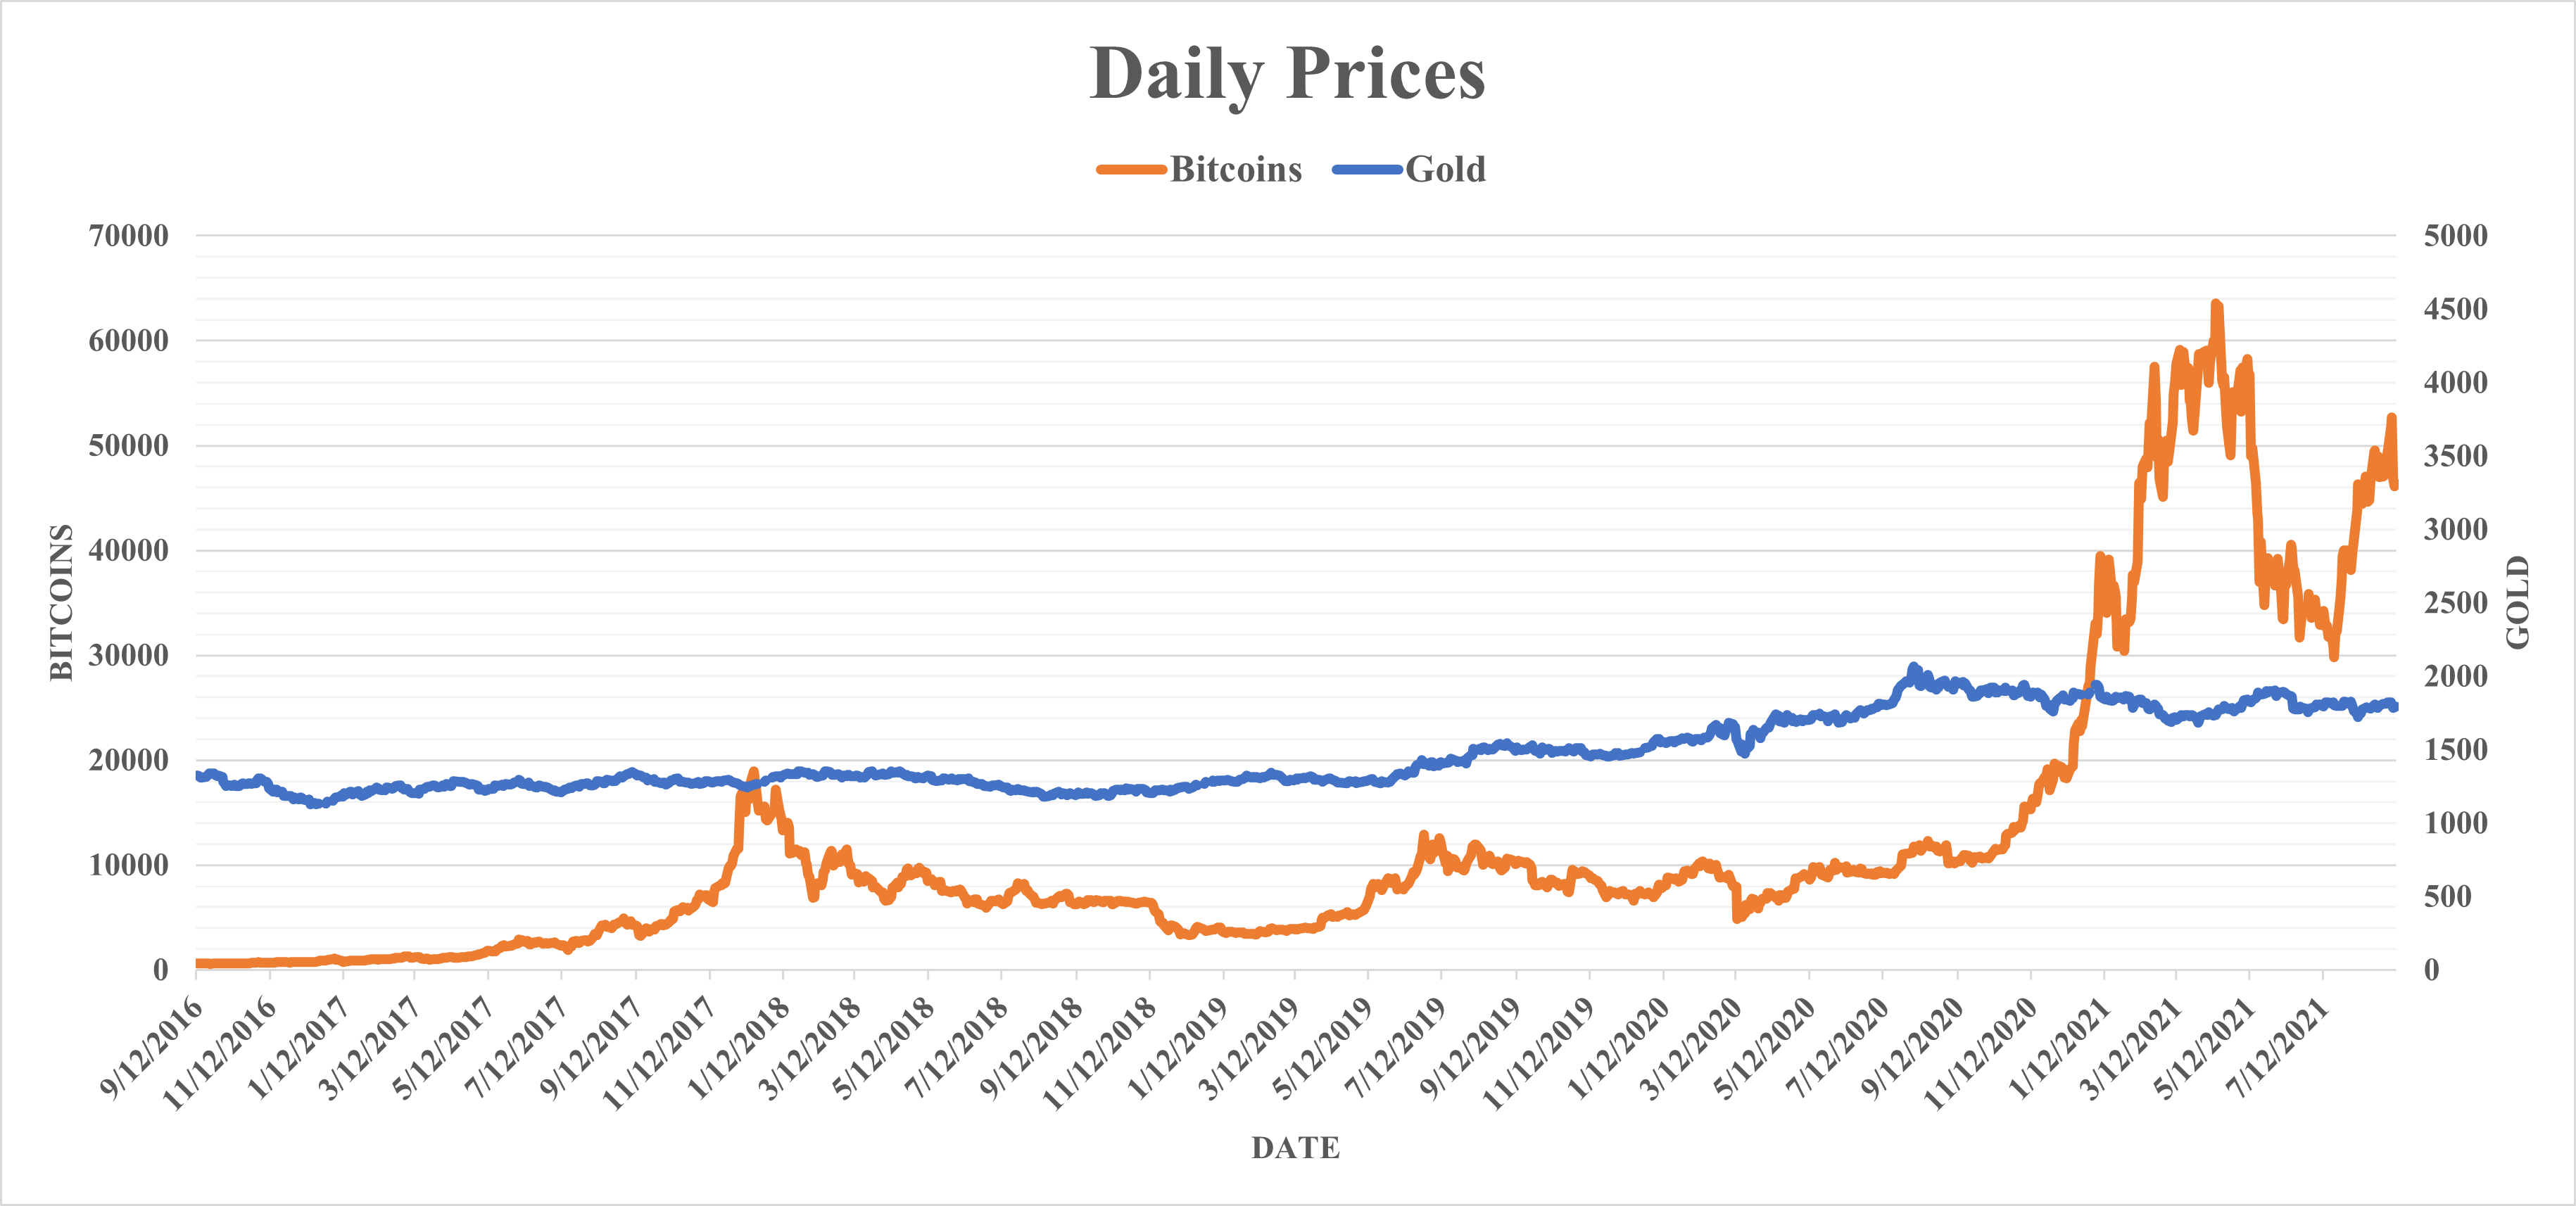
\includegraphics[width=17.0cm]{figures/prices_2in1.png}}
	\caption{Gold and bitcoin daily prices, U.S. dollars per troy ounce and U.S. dollars per bitcoin. Source: London Bullion Market 
		Association, 9/11/2021 and NASDAQ, 9/11/2021 }
	\label{figure:prices2in1}
\end{figure}

\subsection{Restatement of the Problem}

\begin{itemize}
	\item Develop a model that gives the best daily trading strategy based only on price data up 
	to that day, and calculate how much the initial \$1000 investment is worth on 9/10/2021 using the 
	model and strategy.
	
	\item Present evidence that your model provides the best strategy.
	
	\item Determine how sensitive the strategy is to transaction costs and analyze how transaction costs
	affect the strategy and results.
	
\end{itemize}

\subsection{Our Approach}


%%%%%%%%%%%%%%%%%
\section{Assumptions and Justifications}
\label{Assumptions_Justifications}

\subsection{Assumptions}
To simplify the problem stated above, we make following assumptions, each of which is justified properly: 
\begin{enumerate}
	\item \textbf{The market trader sells all of the gold and bitcoins by the end of the five-year trading period, i.e. 9/10/2021.} Generally, investors cares about funding liquidity. Among cash, gold and bitcoins, only cash can circulate unhindered in the market. So we make this assumption and thus measure the outcome in cash.
\end{enumerate}


\subsection{Symbols and Definitions}

\begin{table}[H]
\renewcommand{\arraystretch}{1.5}
\caption{Symbols and Definitions.}
\label{Table_Symbols}
\begin{center}
{\footnotesize
\begin{tabular}{c c}
\toprule
{Notations} & {Description} \\
\midrule
{$\eta$}    & {1} \\ 
{$\xi$}     & {} \\ 
$P$   & {} \\ 
$r$     & {} \\
$x$     & {} \\ 
$X$     & {} \\ 
$N$    & {} \\ 
$n$     & {} \\ 
\bottomrule
\end{tabular}}
\end{center}
\end{table}


\subsection{Symbols and Definitions}

\begin{table}[h]
\renewcommand{\arraystretch}{1.2}
\begin{center}
{\footnotesize
\begin{tabular}{c l}
\toprule
{Notations} & {Description} \\
\midrule
$a$    & {Persuasion of comments} \\
$s(X\rightarrow Y)$  &  {Degree of support between $X$ and $Y$,  indicating how often the rules can be used for analysis}\\
$c(X\rightarrow Y)$  &  {Confidence between $X$ and $Y$, indicating the frequency of transactions in $Y$ containing $X$} \\
$X$ & {Promotion/The `verified purchase' is `N'} \\
$\overline{X}$ & {No promotion or The `verified purchase' is `Y'} \\
$Y$ & {Poor feedback} \\
$\overline{Y}$ & {Favourable feedback} \\
$Z$ & {Poor evaluation support rate} \\
$\overline{Z}$ & {Favourable support rate} \\
$f_{V}$ & {Amount of platform commentators} \\
$f_{\overline{V}}$ & {Amount of common customers} \\
$a_{V}$ & {Support rate of comments written by writers} \\
$a_{\overline{V}}$ & {Support rate of comments written by non writers} \\
$a_{T}$ & {Overall weighted support rate} \\
$Q_\mu(v)$ & {Amount of comments, dependent variable in multiple linear regression} \\
$\mu_i$ & {Regression coefficient of multiple linear regression, $\lbrace i=0, 1, 2, 3 \rbrace$} \\
$v_i$ & {Independent variable of multiple linear regression, $\lbrace i=0, 1, 2, 3 \rbrace$} \\
$v_1$ & {Amount of no promotions in monthly reviews} \\
$v_2$ & {Number of disapproval of poor feedback and approval of favorable feedback in each month} \\
$v_3$ & {Frequency of good keywords in each month} \\
$\xi$ & {Random error term of multiple linear regression} \\
$r^2$ & {Sample determination coefficient discrimination coefficient} \\
$SSR$ & {Regression sum of squares} \\
$SST$ & {Sum of squares of total variation} \\
$T$   & {Weighted mean value of star rating in the train set}\\
$\widetilde{T}$  & {Weighted mean value of star rating in the testing set}\\
$\textbf{std}$  &  {Standard deviation of the result in training set and testing set}\\
$D$ & {Future value of products} \\
$\varphi$ & {Weighted star rating} \\
$\delta$ & {The rate of positive keywords in reviews} \\
\bottomrule
\end{tabular}}
\end{center}
\end{table}



%%%%%%%%%%%%%%%%%
\section{Mathematical Models}
\label{MathModels}


\subsection{Basic Model}

\begin{equation}
\sum\limits_t
\label{Eqn:1}
\end{equation}

According to Equation (\ref{Eqn:1})

\begin{equation}
\left\{ {\begin{array}{*{20}{l}}
{\frac{{d{S_2}}}{{dt}} =  - {R_0} \cdot {S_2}({I_1} + {I_2})}\\
{\frac{{d{I_2}}}{{dt}} = {R_0} \cdot {S_2}({I_1} + {I_2}) - \frac{{{I_2}}}{r}}\\
{\frac{{d{S_1}}}{{dt}} = \rho \left[ {1 - \frac{{{S_1} + (1 + v/r){I_1}}}{{{K_1}}}} \right] - {R_0} \cdot {S_1}({I_1} + {I_2}) - v \cdot {S_1}}\\
{\frac{{d{I_1}}}{{dt}} = {R_0} \cdot {S_1}({I_1} + {I_2}) - \frac{{{I_1}}}{{r + v}}}
\end{array}} \right.
\end{equation}

\subsection{Improved Model}

Additional assumptions for the model improvement


%%  Pseudo-code
\begin{algorithm}  
    \caption{Competitive selection}  
    \label{CompetitiveSeedSelectionAlgorithm}
    
    \KwIn{{the set of data patterns $\mathbb{X}$} }
    \KwOut{the set of prototype seeds $\mathbb{S}^*$}
    Compute the Euclidean distance $dist \left( {\bold{x}_m}, {\bold{x}_n} \right)$ \\  
    Compute the density $D( {\bold{x}_m} ) \ge \gamma$ \\ 
    Select eligible $\bold{x}_m$ for the candidate seed set $\mathbb{C}^0 \gets \left\{  \bold{x}_m \left| \; C( {\bold{x}_m}, \gamma ) = 1\right. \right\}$ \\ 
    Initialize $\mathbb{C}^* \gets \mathbb{C}^0$\\
    \While{$\mathbb{C}^* \neq \phi$}  
    { 
      Initialize $\mathbb{S}^j \gets \mathbb{S}^*$ \\
      Select the winning seed from the candidate set $\bold{x}_s^j \gets \mathop {\arg \max } D({\bold{x}_m})$, ${\bold{x}_m} \in \mathbb{C}^j$ \\
      Update $\mathbb{S}^* \gets \mathbb{S}^j \cup \{ \bold{x}_s^j \}$ \\
      Update $j \gets j + 1$ \\
    }
    return $\mathbb{S}^*$ \\
\end{algorithm} 


%%%%%%%%%%%%%%%%%
\section{Results and Solutions}
\label{Results_Solutions}

Result analysis

Discussions



%%%%%%%%%%%%%%%%%
\section{Model Evaluation and Sensitivity Analysis}
\label{ModelEvaluation_SensitivityAnalysis}



\subsection{Model Evaluation}


\begin{figure}[H]
\centering{
\includegraphics[width=8.0cm]{Figure_MCM_ICM_Flyer.png}}
\caption{Figure illustration.}
\label{Figure_Flyer}
\end{figure}



\subsection{Sensitivity Analysis}


%%%%%%%%%%%%%%%%%
\section{Strength and Weakness}
\label{Strength_Weakness}


\subsection{Strength}

The models have the following strengths:

\begin{itemize}
\item Advantage 1

\item Advantage 2
\end{itemize}


\subsection{Weakness}

The models have the following weaknesses:

\begin{itemize}
\item Weakness 1

\item Weakness 2
\end{itemize}


%%%%%%%%%%%%%%%%%
\section{Conclusions}
\label{Conclusions}






%%%%%%%%%%%%%%%%%
\newpage
\begin{thebibliography}{00}

%% \bibitem{label}
%% Text of bibliographic item

\bibitem{Pawar2012}
P.~Y.~Pawar and S.~H.~Gawande, ``A Comparative Study on Different Types of Approaches to Text Categorization,'' \textit{International Journal of Machine Learning and Computing}, vol. 2, no. 4, pp. 423-426, 2012.

\bibitem{Pang2005}
B.~Pang and L.~Lee, ``Seeing stars: Exploiting class relationships for sentiment categorization with respect to rating scales,'' \textit{Proceedings of the 43rd Meeting of the Association for Computational Linguistics}, pp. 115–124, 2005.

\bibitem{McAuley2013}
J.~McAuley, J.~Leskovec, ``Hidden factors and hidden topics: understanding rating dimensions with review text'', \textit{Proceedings of the 7th ACM Conference on Recommender Systems (RecSys 2013)}, pp. 165-172, October 2013.

\bibitem{Hu2009}
N.~Hu, P.~Pavlou, and J.~Zhang, ``Overcoming the J-shaped distribution of products reviews,'' \textit{Communications of the ACM}, vol. 52, pp. 144-147, 2009. 

\bibitem{Koren2009}
Y.~Koren, R.~Bell, and C.~Volinsky, ``Matrix factorization techniques for recommender systems,'' \textit{Computer}, vol. 42, no. 8, pp. 30-37, 2009.

\bibitem{Hu2008}
Y.~F.~Hu, Y.~Koren, C.~Volinsky, ``Collaborative filtering for implicit feedback datasets,'' \textit{Proceedings of IEEE International Conference on Data Mining (ICDM 2008)}, pp. 263-272, 2008.

\bibitem{Frees2009}
E.~W.~Frees, \textit{Regression Modeling with Actuarial and Financial Applications}, Cambridge, UK: Cambridge University Press, 2009. ISBN: 978-0521135962

\end{thebibliography}
\addcontentsline{toc}{section}{References}


\addtocounter{page}{-1}
\thispagestyle{empty}

%%%%%%%%%%%%%%%%%
\newpage
\addtocounter{page}{-1}
\thispagestyle{empty}

{\centering\section*{Memorandum to the Trader}}

Write the letter here.



\end{spacing}


%%%%%%%%%%%%%%%%%
\newpage
%% The Appendices part is started with the command \appendix;
%% appendix sections are then done as normal sections
\appendix
\addtocounter{page}{-1}
\thispagestyle{empty}



\section*{Appendix: Programs and Codes}

If you do not want to provide program codes, delete this appendix section.
\\

\lstset{
 columns=fixed,       
 numbers=left,                                        % 在左侧显示行号
 numberstyle=\tiny\color{gray},                       % 设定行号格式
 frame=single,                                         % 显示背景边框
 backgroundcolor=\color[RGB]{245,245,244},            % 设定背景颜色
 keywordstyle=\color[RGB]{40,40,255},                 % 设定关键字颜色
 numberstyle=\footnotesize\color{darkgray},           
 commentstyle=\it\color[RGB]{0,96,96},                % 设置代码注释的格式
 stringstyle=\rmfamily\slshape\color[RGB]{128,0,0},   % 设置字符串格式
 showstringspaces=false,                              % 不显示字符串中的空格
 language=python,                                        % 设置语言
}

\begin{minipage}{1\linewidth}
\small{
\begin{lstlisting}
import numpy as np
import matplotlib.pyplot as plt

x = np.array([-3.0, -2.9, -2.8, -2.7, -2.5, -2.4, -2.3, -2.2, -2.1, -2])
y = np.sin(x)

plt.figure()
plt.xlabel("x axis")
plt.ylabel("y axis")
plt.plot(x, y, '-^')
plt.xlim(min(x)-0.05, max(x)+0.05)
plt.ylim(min(y)-0.05, max(y)+0.05)
plt.legend(loc='best')
plt.show()
\end{lstlisting}
}
\end{minipage}


\end{document}


%% End of template
